%
\section{Результаты расчетов тестовых задач}
%
В соответствии с~ описанной математической моделью были проведены расчеты
нескольких тестовых задач, результаты которых качественно верно описывают
рассматриваемые явления. Проверить согласованность результатов расчетов с~
экспериментом пока не представляется возможным.

\subsection{Задача о закачке газа под давлением}
Рассмотрим одномерную модельную задачу фильтрации. Пористость и
абсолютная проницаемость породы постоянны во всем объеме:  $m$=0.4,\; $K=6.64\cdot 10^{-11}$ м$^2$.
Начальные условия:\; $S_w=0.4$,\; $S_n=0.3$,\; $S_g=0.3$, 
$P_w=P_\text{атм}+\rho g h$($h$ - глубина, отсчитывается от верхнего края области);
$T=285K$. Граничные условия:

Сравним, как проходит процесс при двух различных граничных
условиях на температуру:
\begin{equation} \label{noT} \left.T\right|_{x=0}=\left.T\right|_{x=1}=285K; \end{equation}
\begin{equation} \label{T} \left.T\right|_{x=0}=320K,\quad \Biggl.\dfrac{\partial{T}}{\partial{x}}\Biggr|_{x=1}=0. \end{equation}

Результаты расчетов представлены в виде зависимостей профилей насыщенностей фаз,
распределения давления и температуры от~ времени.

По~ оси $x$ отложено расстояние по вертикали от дна резервуара. По~ оси $y$--
значения насыщенностей каждой из фаз на расстоянии $x$ от~ дна резервуара
в~ определенный момент расчетного времени.

\begin{figure}
\begin{center}
\begin{minipage}[h]{0.49\textwidth}
\begin{tikzpicture}
  \begin{axis}[legend entries={$S_w$,$S_n$,$S_g$}, axis lines=left, ymax=1, ymin=0, enlargelimits=true, grid=major, width=1\textwidth, xlabel={$x$, м}, ylabel={$S$}]
    \pgfplotstableread[skip first n=3]{data/test1_1/F-000000005000.tec}{\mytable}
    \addplot [blue, ultra thick] table [x expr=1-\thisrow{0}, y=1] {\mytable};
    \addplot [black, ultra thick] table [x expr=1-\thisrow{0}, y=2] {\mytable};
    \addplot [red, ultra thick] table [x expr=1-\thisrow{0}, y=3] {\mytable};
  \end{axis}
\end{tikzpicture}
\caption{Насыщенности в момент времени $t=5000$с, граничные условия \ref{noT}}
\end{minipage}
\hfill
\begin{minipage}[h]{0.49\textwidth}
\begin{tikzpicture}
  \begin{axis}[legend entries={$S_w$,$S_n$,$S_g$}, axis lines=left, ymax=1, ymin=0, enlargelimits=true, grid=major, width=1\textwidth, xlabel={$x$, м}, ylabel={$S$}]
    \pgfplotstableread[skip first n=3]{data/test1/F-000000005000.tec}{\mytable}
    \addplot [blue, ultra thick] table [x expr=1-\thisrow{0}, y=1] {\mytable};
    \addplot [black, ultra thick] table [x expr=1-\thisrow{0}, y=2] {\mytable};
    \addplot [red, ultra thick] table [x expr=1-\thisrow{0}, y=3] {\mytable};
  \end{axis}
\end{tikzpicture}
\caption{Насыщенности в момент времени $t=5000$с, граничные условия \ref{T}}
\end{minipage}
\vfill
\begin{minipage}[h]{0.49\textwidth}
\begin{tikzpicture}
  \begin{axis}[axis lines=left, ymax=110000, ymin=100000, enlargelimits=true, grid=major, width=1\textwidth, xlabel={$x$, м}, ylabel={$P$, Па}]
    \pgfplotstableread[skip first n=3]{data/test1_1/F-000000005000.tec}{\mytable}
    \addplot [blue, ultra thick] table [x expr=1-\thisrow{0}, y=4] {\mytable};
  \end{axis}
\end{tikzpicture}
\caption{Давление $P_w$ в момент времени $t=5000$с, граничные условия \ref{noT}}
\end{minipage}
\hfill
\begin{minipage}[h]{0.49\textwidth}
\begin{tikzpicture}
  \begin{axis}[axis lines=left, ymax=110000, ymin=100000, enlargelimits=true, grid=major, width=1\textwidth, xlabel={$x$, м}, ylabel={$P$, Па}]
    \pgfplotstableread[skip first n=3]{data/test1/F-000000005000.tec}{\mytable}
    \addplot [blue, ultra thick] table [x expr=1-\thisrow{0}, y=4] {\mytable};
  \end{axis}
\end{tikzpicture}
\caption{Давление $P_w$ в момент времени $t=5000$с, граничные условия \ref{T}}
\end{minipage}
\vfill
\begin{minipage}[h]{0.49\textwidth}
\begin{tikzpicture}
  \begin{axis}[axis lines=left, ymax=320, ymin=285, enlargelimits=true, grid=major, width=1\textwidth, xlabel={$x$, м}, ylabel={$T$, К}]
    \pgfplotstableread[skip first n=3]{data/test1_1/F-000000005000.tec}{\mytable}
    \addplot [blue, ultra thick] table [x expr=1-\thisrow{0}, y=5] {\mytable};
  \end{axis}
\end{tikzpicture}
\caption{Температура в момент времени $t=5000$с, граничные условия \ref{noT}}
\end{minipage}
\hfill
\begin{minipage}[h]{0.49\textwidth}
\begin{tikzpicture}
  \begin{axis}[axis lines=left, ymax=320, ymin=285, enlargelimits=true, grid=major, width=1\textwidth, xlabel={$x$, м}, ylabel={$T$, К}]
    \pgfplotstableread[skip first n=3]{data/test1/F-000000005000.tec}{\mytable}
    \addplot [blue, ultra thick] table [x expr=1-\thisrow{0}, y=5] {\mytable};
  \end{axis}
\end{tikzpicture}
\caption{Температура в момент времени $t=5000$с, граничные условия \ref{T}}
\end{minipage}
\end{center}
\end{figure}

\begin{figure}
\begin{center}
\begin{minipage}[h]{0.49\textwidth}
\begin{tikzpicture}
  \begin{axis}[legend entries={$S_w$,$S_n$,$S_g$}, axis lines=left, ymax=1, ymin=0, enlargelimits=true, grid=major, width=1\textwidth, xlabel={$x$, м}, ylabel={$S$}]
    \pgfplotstableread[skip first n=3]{data/test1_1/F-000000025000.tec}{\mytable}
    \addplot [blue, ultra thick] table [x expr=1-\thisrow{0}, y=1] {\mytable};
    \addplot [black, ultra thick] table [x expr=1-\thisrow{0}, y=2] {\mytable};
    \addplot [red, ultra thick] table [x expr=1-\thisrow{0}, y=3] {\mytable};
  \end{axis}
\end{tikzpicture}
\caption{Насыщенности в момент времени $t=25000$с, граничные условия \ref{noT}}
\end{minipage}
\hfill
\begin{minipage}[h]{0.49\textwidth}
\begin{tikzpicture}
  \begin{axis}[legend entries={$S_w$,$S_n$,$S_g$}, axis lines=left, ymax=1, ymin=0, enlargelimits=true, grid=major, width=1\textwidth, xlabel={$x$, м}, ylabel={$S$}]
    \pgfplotstableread[skip first n=3]{data/test1/F-000000025000.tec}{\mytable}
    \addplot [blue, ultra thick] table [x expr=1-\thisrow{0}, y=1] {\mytable};
    \addplot [black, ultra thick] table [x expr=1-\thisrow{0}, y=2] {\mytable};
    \addplot [red, ultra thick] table [x expr=1-\thisrow{0}, y=3] {\mytable};
  \end{axis}
\end{tikzpicture}
\caption{Насыщенности в момент времени $t=25000$с, граничные условия \ref{T}}
\end{minipage}
\vfill
\begin{minipage}[h]{0.49\textwidth}
\begin{tikzpicture}
  \begin{axis}[axis lines=left, ymax=110000, ymin=100000, enlargelimits=true, grid=major, width=1\textwidth, xlabel={$x$, м}, ylabel={$P$, Па}]
    \pgfplotstableread[skip first n=3]{data/test1_1/F-000000025000.tec}{\mytable}
    \addplot [blue, ultra thick] table [x expr=1-\thisrow{0}, y=4] {\mytable};
  \end{axis}
\end{tikzpicture}
\caption{Давление $P_w$ в момент времени $t=25000$с, граничные условия \ref{noT}}
\end{minipage}
\hfill
\begin{minipage}[h]{0.49\textwidth}
\begin{tikzpicture}
  \begin{axis}[axis lines=left, ymax=110000, ymin=100000, enlargelimits=true, grid=major, width=1\textwidth, xlabel={$x$, м}, ylabel={$P$, Па}]
    \pgfplotstableread[skip first n=3]{data/test1/F-000000025000.tec}{\mytable}
    \addplot [blue, ultra thick] table [x expr=1-\thisrow{0}, y=4] {\mytable};
  \end{axis}
\end{tikzpicture}
\caption{Давление $P_w$ в момент времени $t=25000$с, граничные условия \ref{T}}
\end{minipage}
\vfill
\begin{minipage}[h]{0.49\textwidth}
\begin{tikzpicture}
  \begin{axis}[axis lines=left, ymax=320, ymin=285, enlargelimits=true, grid=major, width=1\textwidth, xlabel={$x$, м}, ylabel={$T$, К}]
    \pgfplotstableread[skip first n=3]{data/test1_1/F-000000025000.tec}{\mytable}
    \addplot [blue, ultra thick] table [x expr=1-\thisrow{0}, y=5] {\mytable};
  \end{axis}
\end{tikzpicture}
\caption{Температура в момент времени $t=25000$с, граничные условия \ref{noT}}
\end{minipage}
\hfill
\begin{minipage}[h]{0.49\textwidth}
\begin{tikzpicture}
  \begin{axis}[axis lines=left, ymax=320, ymin=285, enlargelimits=true, grid=major, width=1\textwidth, xlabel={$x$, м}, ylabel={$T$, К}]
    \pgfplotstableread[skip first n=3]{data/test1/F-000000025000.tec}{\mytable}
    \addplot [blue, ultra thick] table [x expr=1-\thisrow{0}, y=5] {\mytable};
  \end{axis}
\end{tikzpicture}
\caption{Температура в момент времени $t=25000$с, граничные условия \ref{T}}
\end{minipage}
\end{center}
\end{figure}

\subsection{Задача о перераспределении фаз под действием силы тяжести}
Рассмотрим одномерную модельную задачу фильтрации. Пористость и~
абсолютная проницаемость породы постоянны во~ всем объеме:  $m$=0.4,\; $K=6.64\cdot 10^{-11}$ м$^2$.
Начальные условия:\; $S_w=0.4$,\; $S_n=0.3$,\; $S_g=0.3$, 
$P_w=P_\text{атм}+\rho g h$($h$ - глубина, отсчитывается от~ верхнего края области);
$T=285K$. Граничные условия:

$\left.T\right|_{x=0}=320K, \left.T\right|_{x=1}=285K;$
$\left.P\right|_{x=0}=P_{\text{атм}},\quad \Biggl.\dfrac{\partial{P_w}}{\partial{x}}\Biggr|_{x=1}=0;$
$\left.S_w\right|_{x=0}=0.01,\quad \Biggl.\dfrac{\partial{S_w}}{\partial{x}}\Biggr|_{x=1}=0;$
$\left.S_n\right|_{x=0}=0.01,\quad \Biggl.\dfrac{\partial{S_n}}{\partial{x}}\Biggr|_{x=1}=0;$

Результаты расчетов представлены в~ виде зависимостей профилей насыщенностей фаз,
распределения давления и~ температуры от~ времени.

По~ оси $x$ отложено расстояние по вертикали от дна резервуара. По~ оси $y$--
значения насыщенностей каждой из~ фаз на~ расстоянии $x$ от~ дна резервуара
в~ определенный момент расчетного времени.

\begin{figure}
\begin{center}
\begin{minipage}[h]{0.49\textwidth}
\begin{tikzpicture}
  \begin{axis}[legend entries={$S_w$,$S_n$,$S_g$}, axis lines=left, ymax=1, ymin=0, enlargelimits=true, grid=major, width=1\textwidth, xlabel={$x$, м}, ylabel={$S$}]
    \pgfplotstableread[skip first n=3]{data/test2/F-000000004000.tec}{\mytable}
    \addplot [blue, ultra thick] table [x expr=1-\thisrow{0}, y=1] {\mytable};
    \addplot [black, ultra thick] table [x expr=1-\thisrow{0}, y=2] {\mytable};
    \addplot [red, ultra thick] table [x expr=1-\thisrow{0}, y=3] {\mytable};
  \end{axis}
\end{tikzpicture}
\caption{Насыщенности в момент времени $t=4000$с}
\end{minipage}
\hfill
\begin{minipage}[h]{0.49\textwidth}
\begin{tikzpicture}
  \begin{axis}[legend entries={$S_w$,$S_n$,$S_g$}, axis lines=left, ymax=1, ymin=0, enlargelimits=true, grid=major, width=1\textwidth, xlabel={$x$, м}, ylabel={$S$}]
    \pgfplotstableread[skip first n=3]{data/test2/F-000000010000.tec}{\mytable}
    \addplot [blue, ultra thick] table [x expr=1-\thisrow{0}, y=1] {\mytable};
    \addplot [black, ultra thick] table [x expr=1-\thisrow{0}, y=2] {\mytable};
    \addplot [red, ultra thick] table [x expr=1-\thisrow{0}, y=3] {\mytable};
  \end{axis}
\end{tikzpicture}
\caption{Насыщенности в момент времени $t=10000$с}
\end{minipage}
\vfill
\begin{minipage}[h]{0.49\textwidth}
\begin{tikzpicture}
  \begin{axis}[axis lines=left, ymax=105000, ymin=100000, enlargelimits=true, grid=major, width=1\textwidth, xlabel={$x$, м}, ylabel={$P$, Па}]
    \pgfplotstableread[skip first n=3]{data/test2/F-000000004000.tec}{\mytable}
    \addplot [blue, ultra thick] table [x expr=1-\thisrow{0}, y=4] {\mytable};
  \end{axis}
\end{tikzpicture}
\caption{Давление $P_w$ в момент времени $t=4000$с}
\end{minipage}
\hfill
\begin{minipage}[h]{0.49\textwidth}
\begin{tikzpicture}
  \begin{axis}[axis lines=left, ymax=105000, ymin=100000, enlargelimits=true, grid=major, width=1\textwidth, xlabel={$x$, м}, ylabel={$P$, Па}]
    \pgfplotstableread[skip first n=3]{data/test2/F-000000010000.tec}{\mytable}
    \addplot [blue, ultra thick] table [x expr=1-\thisrow{0}, y=4] {\mytable};
  \end{axis}
\end{tikzpicture}
\caption{Давление $P_w$ в момент времени $t=10000$с}
\end{minipage}
\vfill
\begin{minipage}[h]{0.49\textwidth}
\begin{tikzpicture}
  \begin{axis}[axis lines=left, ymax=320, ymin=285, enlargelimits=true, grid=major, width=1\textwidth, xlabel={$x$, м}, ylabel={$T$, К}]
    \pgfplotstableread[skip first n=3]{data/test2/F-000000004000.tec}{\mytable}
    \addplot [blue, ultra thick] table [x expr=1-\thisrow{0}, y=5] {\mytable};
  \end{axis}
\end{tikzpicture}
\caption{Температура в момент времени $t=4000$с}
\end{minipage}
\hfill
\begin{minipage}[h]{0.49\textwidth}
\begin{tikzpicture}
  \begin{axis}[axis lines=left, ymax=320, ymin=285, enlargelimits=true, grid=major, width=1\textwidth, xlabel={$x$, м}, ylabel={$T$, К}]
    \pgfplotstableread[skip first n=3]{data/test2/F-000000010000.tec}{\mytable}
    \addplot [blue, ultra thick] table [x expr=1-\thisrow{0}, y=5] {\mytable};
  \end{axis}
\end{tikzpicture}
\caption{Температура в момент времени $t=10000$с}
\end{minipage}
\end{center}
\end{figure}

\subsection{Двухмерная задача просачивания с источником на границе}
Рассмотрим двумерную область пористой среды, имеющую форму
прямоугольника. Пористость и абсолютная проницаемость породы постоянны во всем
объеме. Параметры модели такие же, как
в первой тестовой задаче.
Во всей области задаем следующее 
начальное распределение: $S_w=0.4$,\; $S_n=0.35$,\; $S_g=0.25$, 
$P_w=P_\text{атм}+\rho g h$($h$ - глубина, отсчитывается от верхнего края области).
Пусть размер области -- $N_x\cdot N_y$.
Граничную поверхность, кроме части верхней границы, считаем непроницаемой, 
что может быть интерпретировано так,
что среда огорожена непроницаемым резервуаром, имеющим сверху отверстие с
координатами: $(N_x/3, N_y)$, $(2N_x/3, N_y)$. Через отверстие происходит обмен веществом между 
резервуаром и окружающей средой. На отверстии заданы условия: $P_w=P_\text{атм}$,

$ \dfrac{\partial S_w}{\partial t}= 
\begin{cases}
 q, \; S_w<S_{max}\\
 0, \; \text{иначе}
\end{cases}
$,
$ \dfrac{\partial S_n}{\partial t}=-q S_n$.

\begin{figure}
\begin{center}
\begin{minipage}[h]{0.48\textwidth}
\begin{tikzpicture}
  \begin{axis}[view={0}{90}, enlargelimits=false, xlabel={$x$, м}, ylabel={$y$, м}, colorbar, width=0.8\textwidth, height=0.8\textwidth, point meta min=100000, point meta max=110000]
    \pgfplotstableread[skip first n=3]{data/test3/F-000000000100.tec}{\mytable}
    \addplot3 [surf, shader=interp] table [x=0, y=1, z=5] {\mytable};
  \end{axis}
\end{tikzpicture}
\caption{Давление $P_w$ в момент времени $t=100$с}
\end{minipage}
\hfill
\begin{minipage}[h]{0.48\textwidth}
\begin{tikzpicture}
  \begin{axis}[view={0}{90}, enlargelimits=false, xlabel={$x$, м}, ylabel={$y$, м}, colorbar, width=0.8\textwidth, height=0.8\textwidth, point meta min=285, point meta max=320]
    \pgfplotstableread[skip first n=3]{data/test3/F-000000000100.tec}{\mytable}
    \addplot3 [surf, shader=interp] table [x=0, y=1, z=6] {\mytable};
  \end{axis}
\end{tikzpicture}
\caption{Температура в момент времени $t=1000$с}
\end{minipage}
\vfill
\begin{minipage}[h]{0.48\textwidth}
\begin{tikzpicture}
  \begin{axis}[view={0}{90}, enlargelimits=false, xlabel={$x$, м}, ylabel={$y$, м}, colorbar, width=0.8\textwidth, height=0.8\textwidth, point meta min=100000, point meta max=110000]
    \pgfplotstableread[skip first n=3]{data/test3/F-000000001000.tec}{\mytable}
    \addplot3 [surf, shader=interp] table [x=0, y=1, z=5] {\mytable};
  \end{axis}
\end{tikzpicture}
\caption{Давление $P_w$ в момент времени $t=1000$с}
\end{minipage}
\hfill
\begin{minipage}[h]{0.48\textwidth}
\begin{tikzpicture}
  \begin{axis}[view={0}{90}, enlargelimits=false, xlabel={$x$, м}, ylabel={$y$, м}, colorbar, width=0.8\textwidth, height=0.8\textwidth, point meta min=285, point meta max=320]
    \pgfplotstableread[skip first n=3]{data/test3/F-000000001000.tec}{\mytable}
    \addplot3 [surf, shader=interp] table [x=0, y=1, z=6] {\mytable};
  \end{axis}
\end{tikzpicture}
\caption{Температура в момент времени $t=1000$с}
\end{minipage}
\vfill
\begin{minipage}[h]{0.48\textwidth}
\begin{tikzpicture}
  \begin{axis}[view={0}{90}, enlargelimits=false, xlabel={$x$, м}, ylabel={$y$, м}, colorbar, width=0.8\textwidth, height=0.8\textwidth, point meta min=100000, point meta max=110000]
    \pgfplotstableread[skip first n=3]{data/test3/F-000000007000.tec}{\mytable}
    \addplot3 [surf, shader=interp] table [x=0, y=1, z=5] {\mytable};
  \end{axis}
\end{tikzpicture}
\caption{Давление $P_w$ в момент времени $t=7000$с}
\end{minipage}
\hfill
\begin{minipage}[h]{0.48\textwidth}
\begin{tikzpicture}
  \begin{axis}[view={0}{90}, enlargelimits=false, xlabel={$x$, м}, ylabel={$y$, м}, colorbar, width=0.8\textwidth, height=0.8\textwidth, point meta min=285, point meta max=320]
    \pgfplotstableread[skip first n=3]{data/test3/F-000000007000.tec}{\mytable}
    \addplot3 [surf, shader=interp] table [x=0, y=1, z=6] {\mytable};
  \end{axis}
\end{tikzpicture}
\caption{Температура в момент времени $t=7000$с}
\end{minipage}
\end{center}
\end{figure}
\begin{figure}
\begin{center}
\begin{minipage}[h]{0.48\textwidth}
\begin{tikzpicture}
  \begin{axis}[view={0}{90}, enlargelimits=false, xlabel={$x$, м}, ylabel={$y$, м}, colorbar, width=0.8\textwidth, height=0.8\textwidth, point meta min=0.1, point meta max=0.6]
    \pgfplotstableread[skip first n=3]{data/test3/F-000000000100.tec}{\mytable}
    \addplot3 [surf, shader=interp] table [x=0, y=1, z=2] {\mytable};
  \end{axis}
\end{tikzpicture}
\caption{Насыщенность $S_w$ в момент времени $t=100$с}
\end{minipage}
\hfill
\begin{minipage}[h]{0.48\textwidth}
\begin{tikzpicture}
  \begin{axis}[view={0}{90}, enlargelimits=false, xlabel={$x$, м}, ylabel={$y$, м}, colorbar, width=0.8\textwidth, height=0.8\textwidth, point meta min=0.1, point meta max=0.48]
    \pgfplotstableread[skip first n=3]{data/test3/F-000000000100.tec}{\mytable}
    \addplot3 [surf, shader=interp] table [x=0, y=1, z=3] {\mytable};
  \end{axis}
\end{tikzpicture}
\caption{Насыщенность $S_n$ в момент времени $t=100$с}
\end{minipage}
\vfill
\begin{minipage}[h]{0.48\textwidth}
\begin{tikzpicture}
  \begin{axis}[view={0}{90}, enlargelimits=false, xlabel={$x$, м}, ylabel={$y$, м}, colorbar, width=0.8\textwidth, height=0.8\textwidth, point meta min=0.1, point meta max=0.6]
    \pgfplotstableread[skip first n=3]{data/test3/F-000000001000.tec}{\mytable}
    \addplot3 [surf, shader=interp] table [x=0, y=1, z=2] {\mytable};
  \end{axis}
\end{tikzpicture}
\caption{Насыщенность $S_w$ в момент времени $t=1000$с}
\end{minipage}
\hfill
\hfill
\begin{minipage}[h]{0.48\textwidth}
\begin{tikzpicture}
  \begin{axis}[view={0}{90}, enlargelimits=false, xlabel={$x$, м}, ylabel={$y$, м}, colorbar, width=0.8\textwidth, height=0.8\textwidth, point meta min=0.1, point meta max=0.48]
    \pgfplotstableread[skip first n=3]{data/test3/F-000000001000.tec}{\mytable}
    \addplot3 [surf, shader=interp] table [x=0, y=1, z=3] {\mytable};
  \end{axis}
\end{tikzpicture}
\caption{Насыщенность $S_n$ в момент времени $t=1000$с}
\end{minipage}
\vfill
\begin{minipage}[h]{0.48\textwidth}
\begin{tikzpicture}
  \begin{axis}[view={0}{90}, enlargelimits=false, xlabel={$x$, м}, ylabel={$y$, м}, colorbar, width=0.8\textwidth, height=0.8\textwidth, point meta min=0.1, point meta max=0.6]
    \pgfplotstableread[skip first n=3]{data/test3/F-000000007000.tec}{\mytable}
    \addplot3 [surf, shader=interp] table [x=0, y=1, z=2] {\mytable};
  \end{axis}
\end{tikzpicture}
\caption{Насыщенность $S_w$ вТемпература момент времени $t=7000$с}
\end{minipage}
\hfill
\begin{minipage}[h]{0.48\textwidth}
\begin{tikzpicture}
  \begin{axis}[view={0}{90}, enlargelimits=false, xlabel={$x$, м}, ylabel={$y$, м}, colorbar, width=0.8\textwidth, height=0.8\textwidth, point meta min=0.1, point meta max=0.48]
    \pgfplotstableread[skip first n=3]{data/test3/F-000000007000.tec}{\mytable}
    \addplot3 [surf, shader=interp] table [x=0, y=1, z=3] {\mytable};
  \end{axis}
\end{tikzpicture}
\caption{Насыщенность $S_n$ в момент времени $t=7000$с}
\end{minipage}
\end{center}
\end{figure}
\begin{figure}
\begin{center}
\begin{minipage}[h]{0.48\textwidth}
\begin{tikzpicture}
  \begin{axis}[view={0}{90}, enlargelimits=false, xlabel={$x$, м}, ylabel={$y$, м}, colorbar, width=0.8\textwidth, height=0.8\textwidth, point meta min=0.1, point meta max=0.48]
    \pgfplotstableread[skip first n=3]{data/test3/F-000000000100.tec}{\mytable}
    \addplot3 [surf, shader=interp] table [x=0, y=1, z=4] {\mytable};
  \end{axis}
\end{tikzpicture}
\caption{Насыщенность $S_g$ в момент времени $t=100$с}
\end{minipage}
\vfill
\begin{minipage}[h]{0.48\textwidth}
\begin{tikzpicture}
  \begin{axis}[view={0}{90}, enlargelimits=false, xlabel={$x$, м}, ylabel={$y$, м}, colorbar, width=0.8\textwidth, height=0.8\textwidth, point meta min=0.1, point meta max=0.48]
    \pgfplotstableread[skip first n=3]{data/test3/F-000000001000.tec}{\mytable}
    \addplot3 [surf, shader=interp] table [x=0, y=1, z=4] {\mytable};
  \end{axis}
\end{tikzpicture}
\caption{Насыщенность $S_g$ в момент времени $t=1000$с}
\end{minipage}
\vfill
\begin{minipage}[h]{0.48\textwidth}
\begin{tikzpicture}
  \begin{axis}[view={0}{90}, enlargelimits=false, xlabel={$x$, м}, ylabel={$y$, м}, colorbar, width=0.8\textwidth, height=0.8\textwidth, point meta min=0.1, point meta max=0.48]
    \pgfplotstableread[skip first n=3]{data/test3/F-000000007000.tec}{\mytable}
    \addplot3 [surf, shader=interp] table [x=0, y=1, z=4] {\mytable};
  \end{axis}
\end{tikzpicture}
\caption{Насыщенность $S_g$ в момент времени $t=7000$с}
\end{minipage}
\end{center}
\end{figure}


\subsection{Трехмерная задача просачивания с источником на границе}

\begin{figure}
  \begin{center}
    \begin{minipage}[h]{0.49\textwidth}
       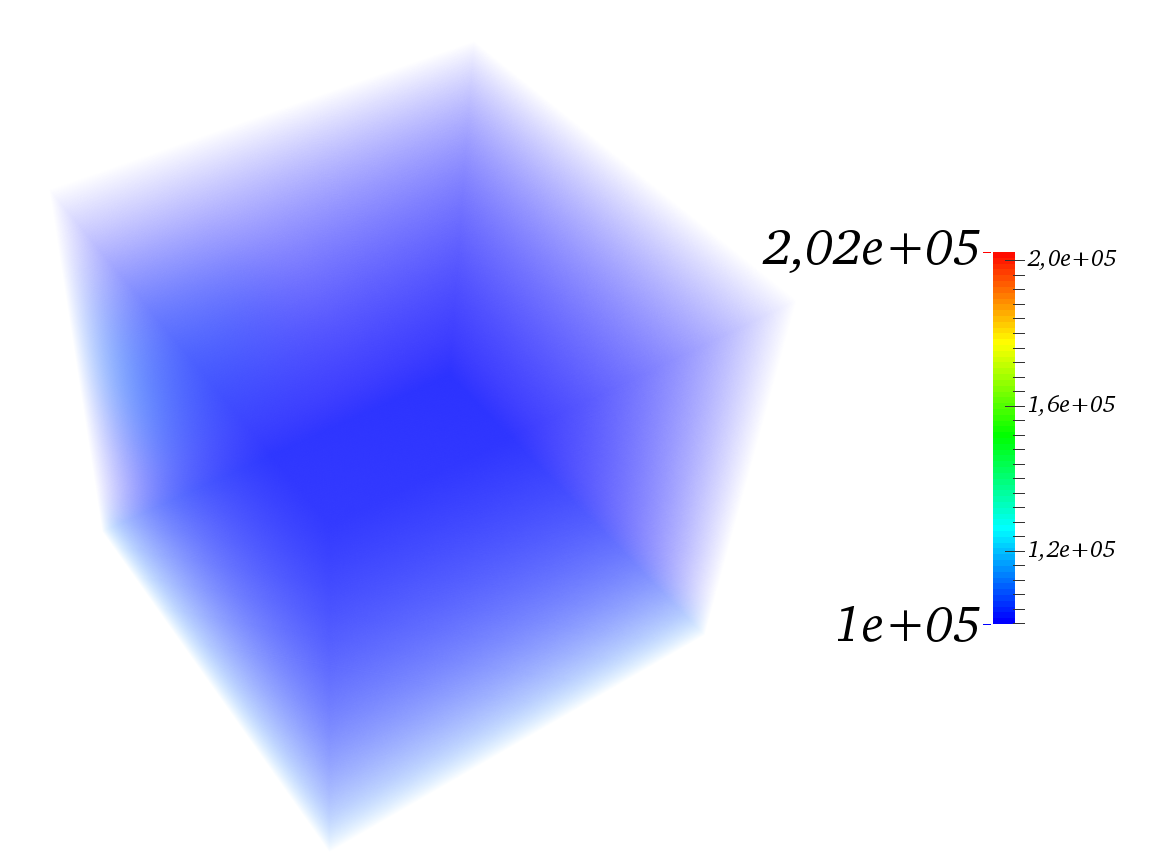
\includegraphics[width=1\textwidth]{test4/pw_200.png}
       \vspace{1cm}
       \caption{Давление $P_w$ в момент времени $t=200$с}
    \end{minipage}
    \hfill
    \begin{minipage}[h]{0.49\textwidth}
       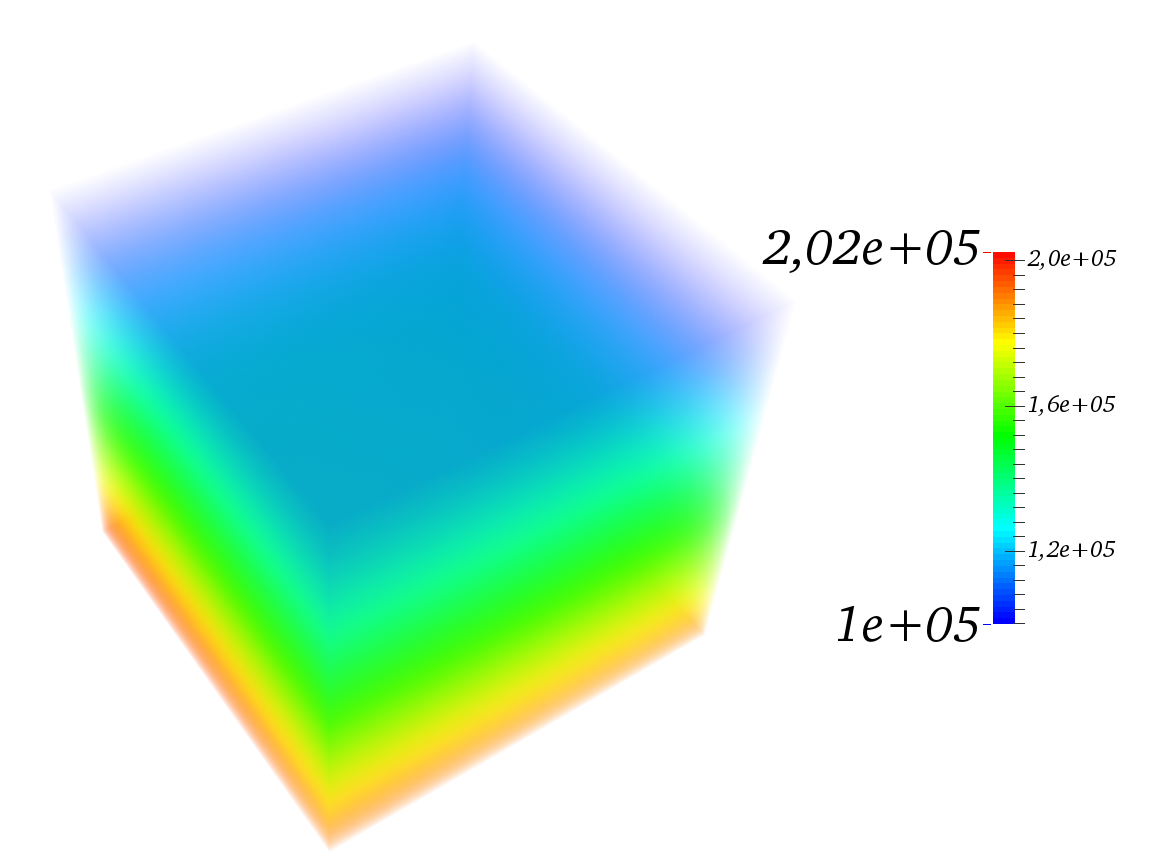
\includegraphics[width=1\textwidth]{test4/pw_1000.png}
       \vspace{1cm}
       \caption{Давление $P_w$ в момент времени $t=1000$с}
    \end{minipage}
    \vspace{3cm}
    \vfill
    \begin{minipage}[h]{0.49\textwidth}
       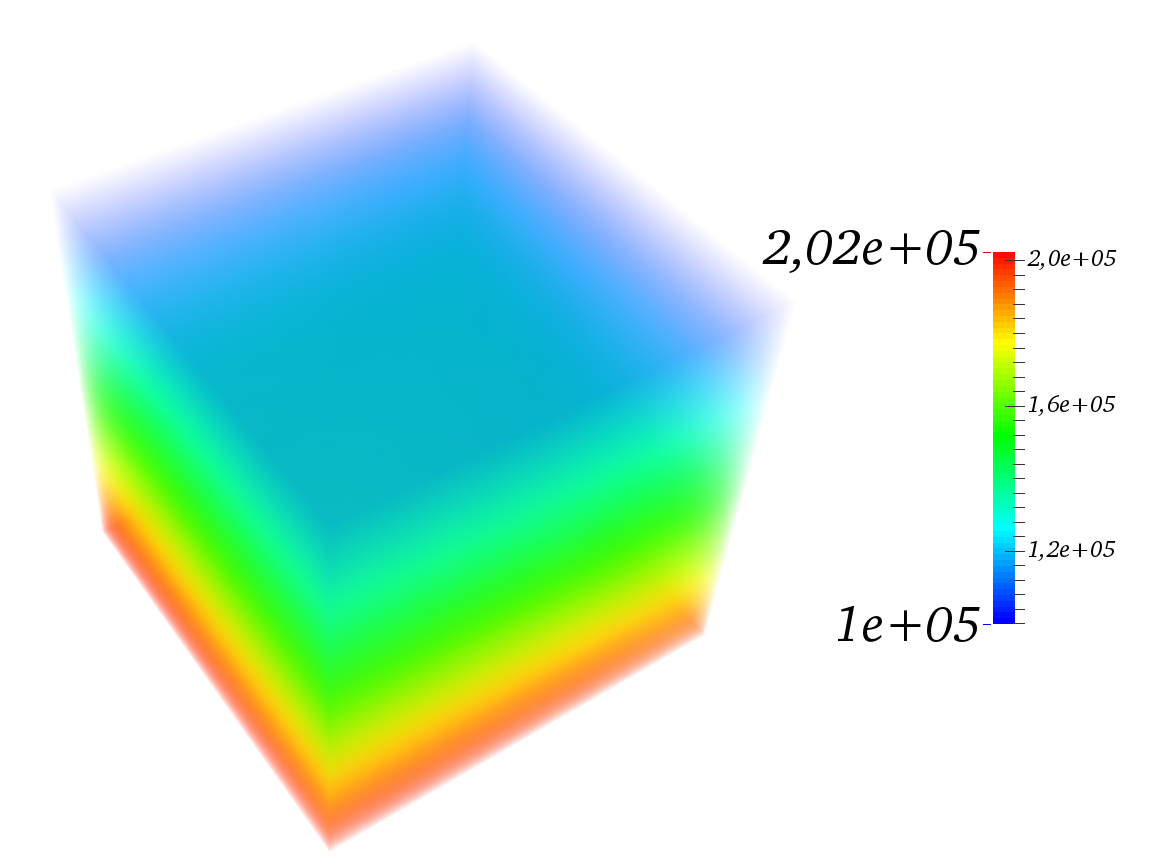
\includegraphics[width=1\textwidth]{test4/pw_2000.png}
       \vspace{1cm}
       \caption{Давление $P_w$ в момент времени $t=2000$с}
    \end{minipage}
    \hfill
    \begin{minipage}[h]{0.49\textwidth}
       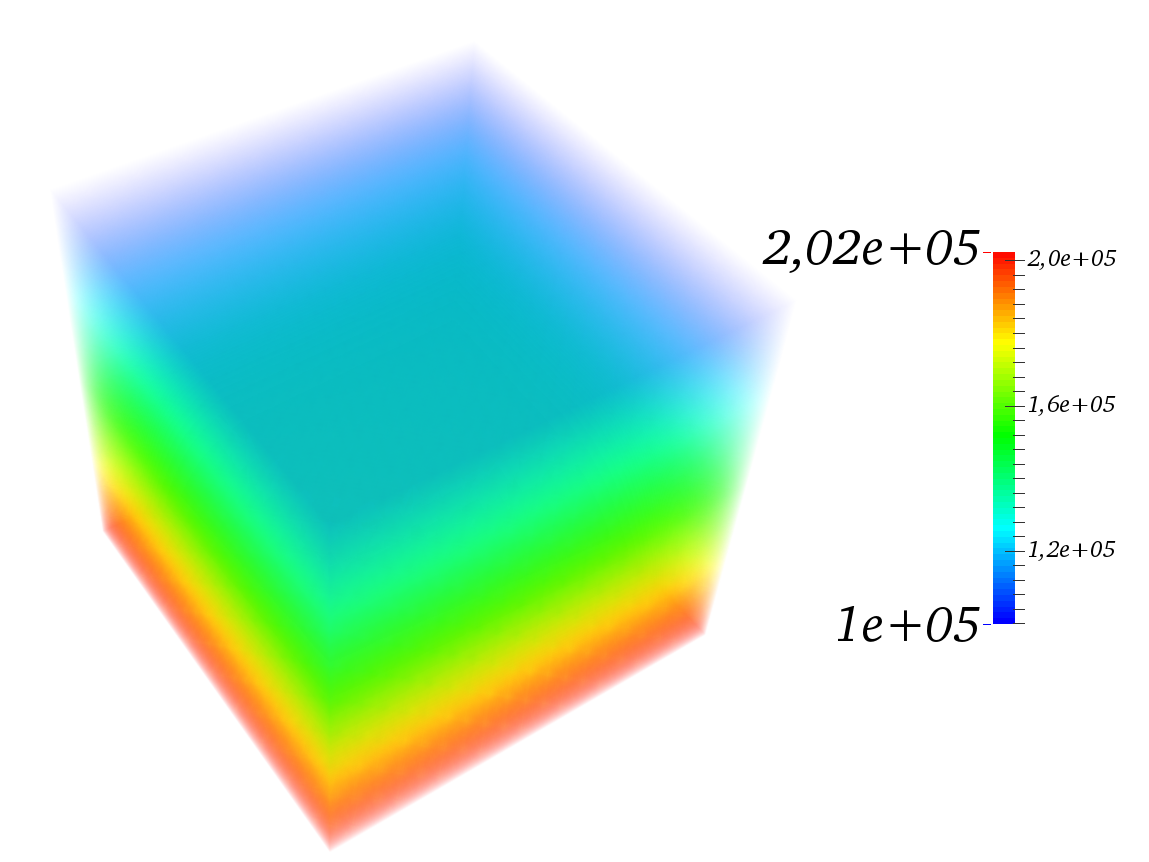
\includegraphics[width=1\textwidth]{test4/pw_6600.png}
       \vspace{1cm}
       \caption{Давление $P_w$ в момент времени $t=6600$с}
    \end{minipage}
    \hfill  
  \end{center}
\end{figure}

\begin{figure}
  \begin{center}
    \begin{minipage}[h]{0.49\textwidth}
       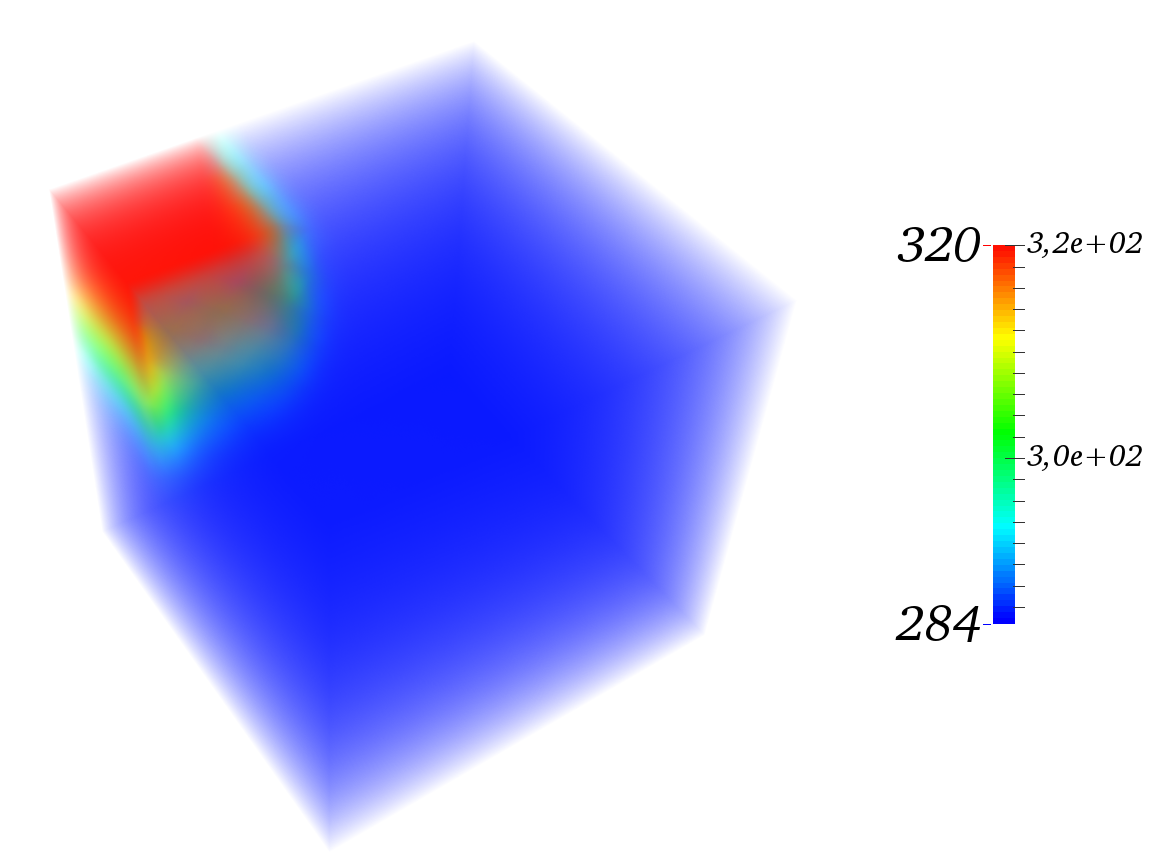
\includegraphics[width=1\textwidth]{test4/t_200.png}
       \vspace{1cm}
       \caption{Температура в момент времени $t=200$с}
    \end{minipage}
    \hfill
    \begin{minipage}[h]{0.49\textwidth}
       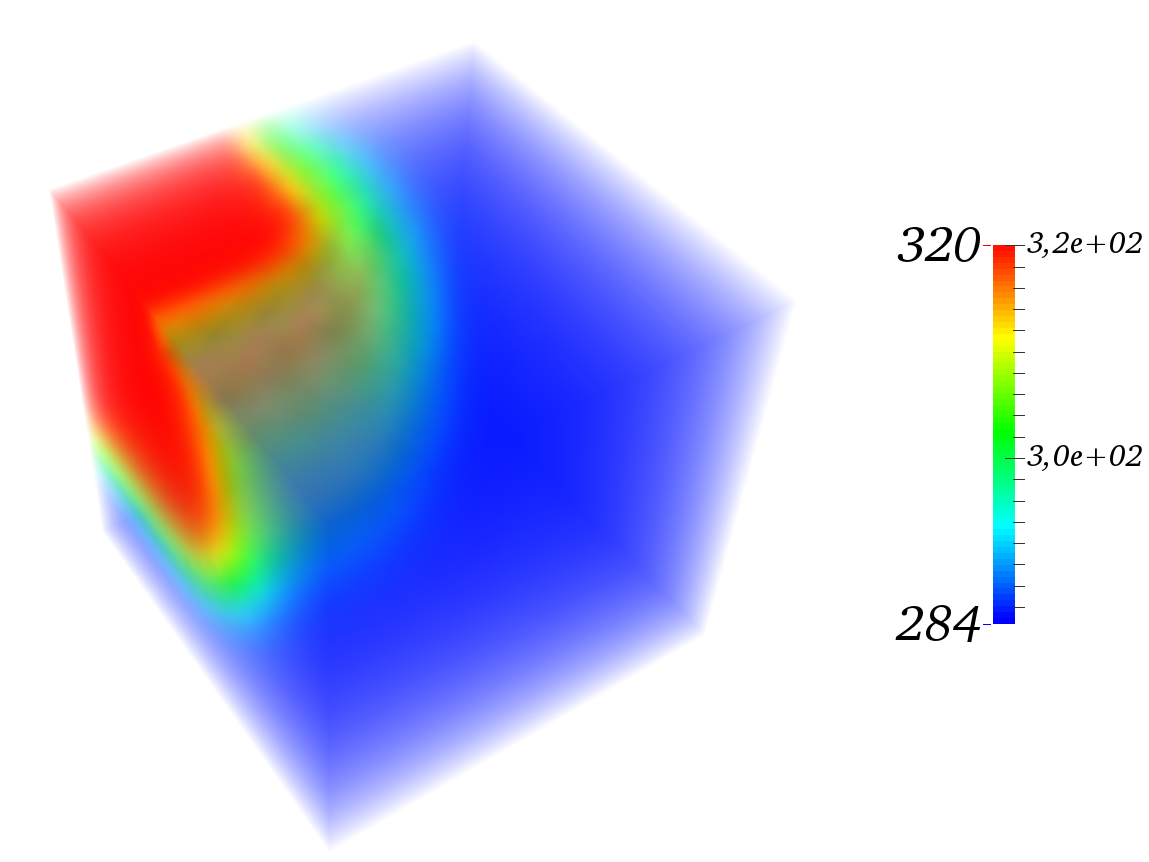
\includegraphics[width=1\textwidth]{test4/t_1000.png}
       \vspace{1cm}
       \caption{Температура в момент времени $t=1000$с}
    \end{minipage}
    \vspace{3cm}
    \vfill
    \begin{minipage}[h]{0.49\textwidth}
       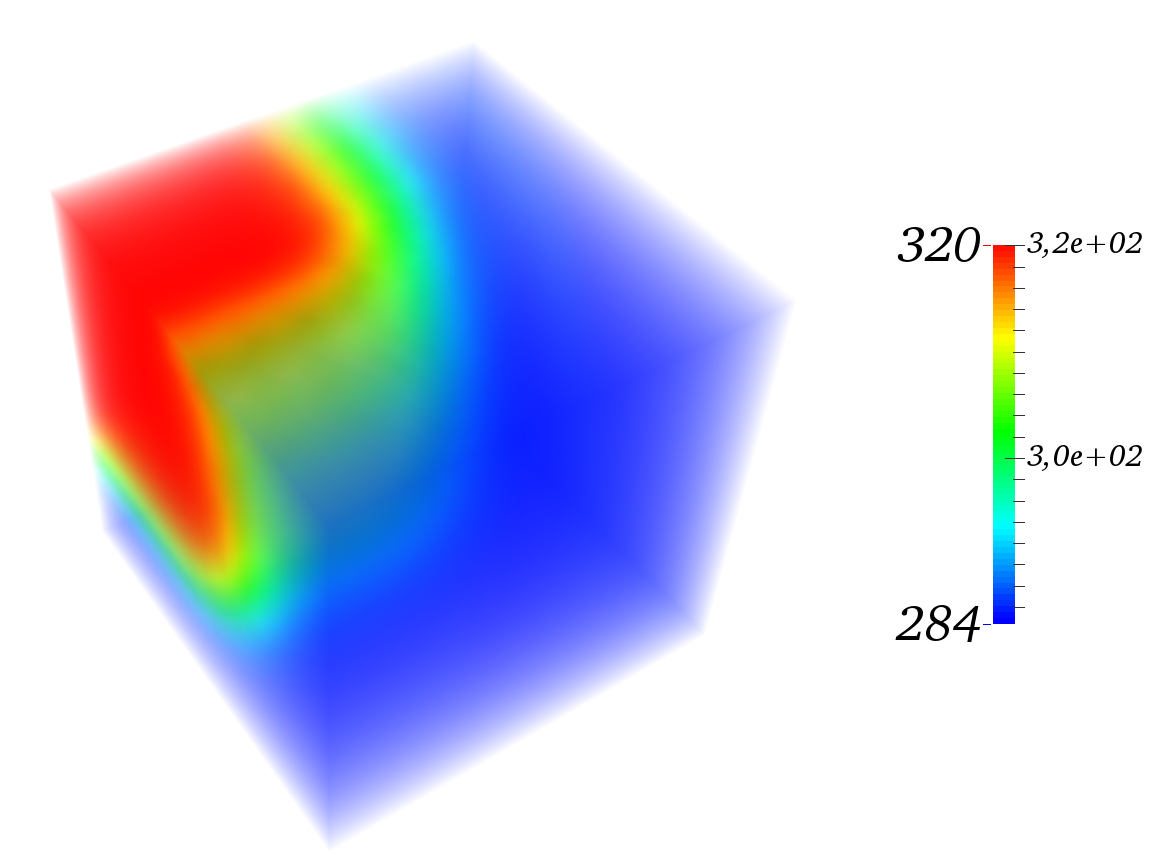
\includegraphics[width=1\textwidth]{test4/t_2000.png}
       \vspace{1cm}
       \caption{Температура в момент времени $t=2000$с}
    \end{minipage}
    \hfill
    \begin{minipage}[h]{0.49\textwidth}
       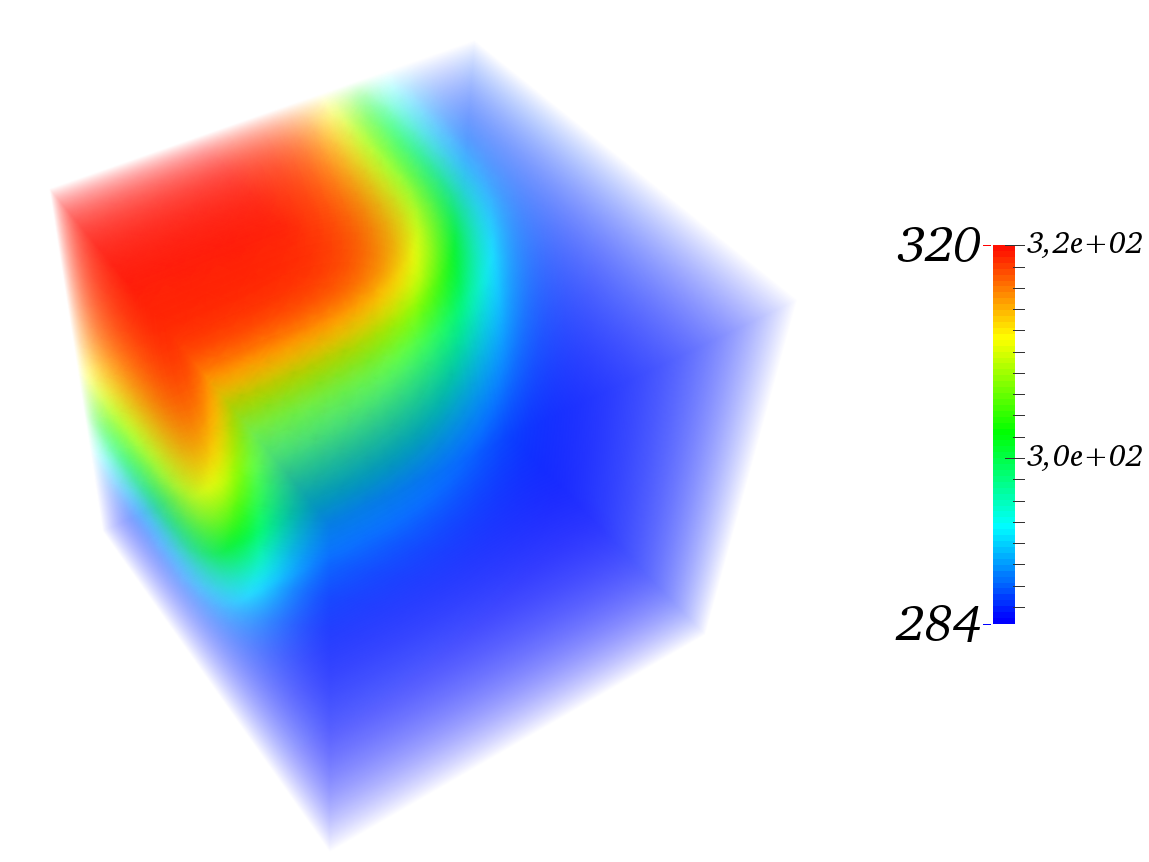
\includegraphics[width=1\textwidth]{test4/t_6600.png}
       \vspace{1cm}
       \caption{Температура в момент времени $t=6600$с}
    \end{minipage}
    \hfill  
  \end{center}
\end{figure}

\begin{figure}
  \begin{center}
    \begin{minipage}[h]{0.49\textwidth}
       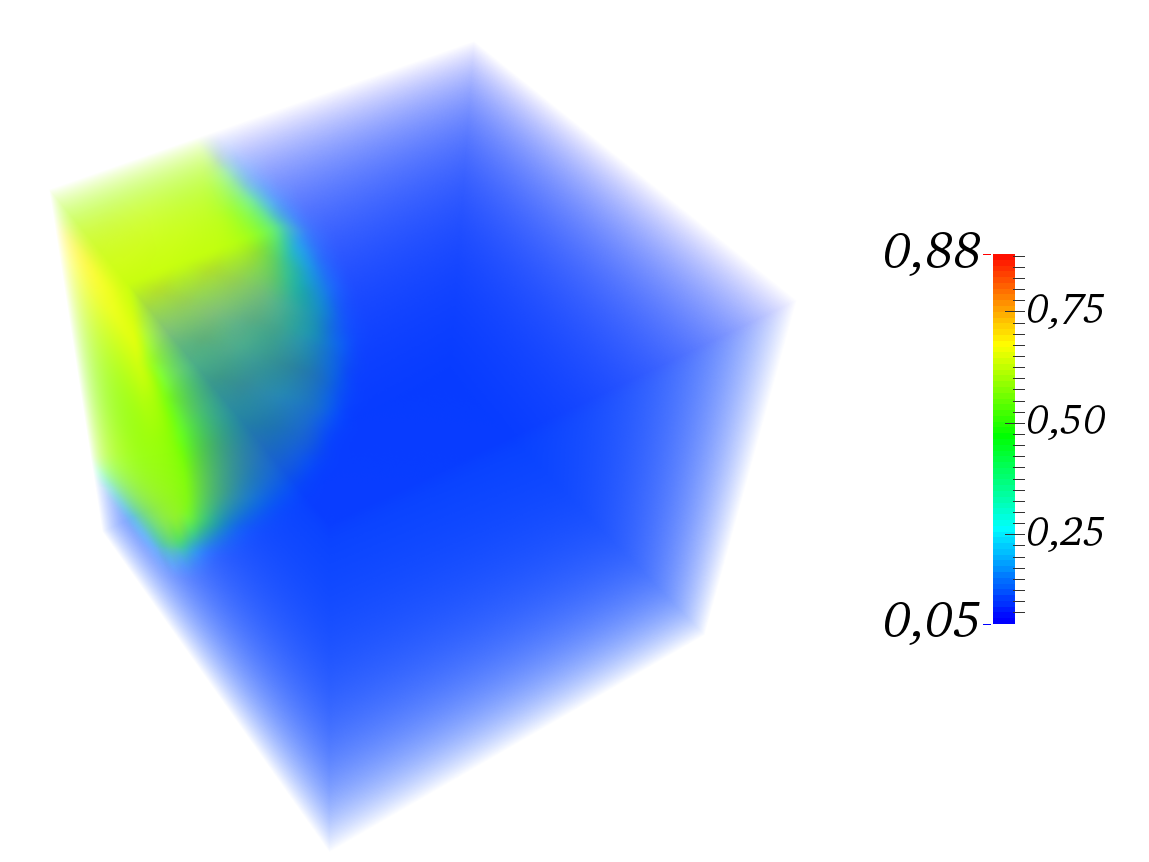
\includegraphics[width=1\textwidth]{test4/sw_200.png}
       \vspace{1cm}
       \caption{Насыщенность $S_w$ в момент времени $t=200$с}
    \end{minipage}
    \hfill
    \begin{minipage}[h]{0.49\textwidth}
       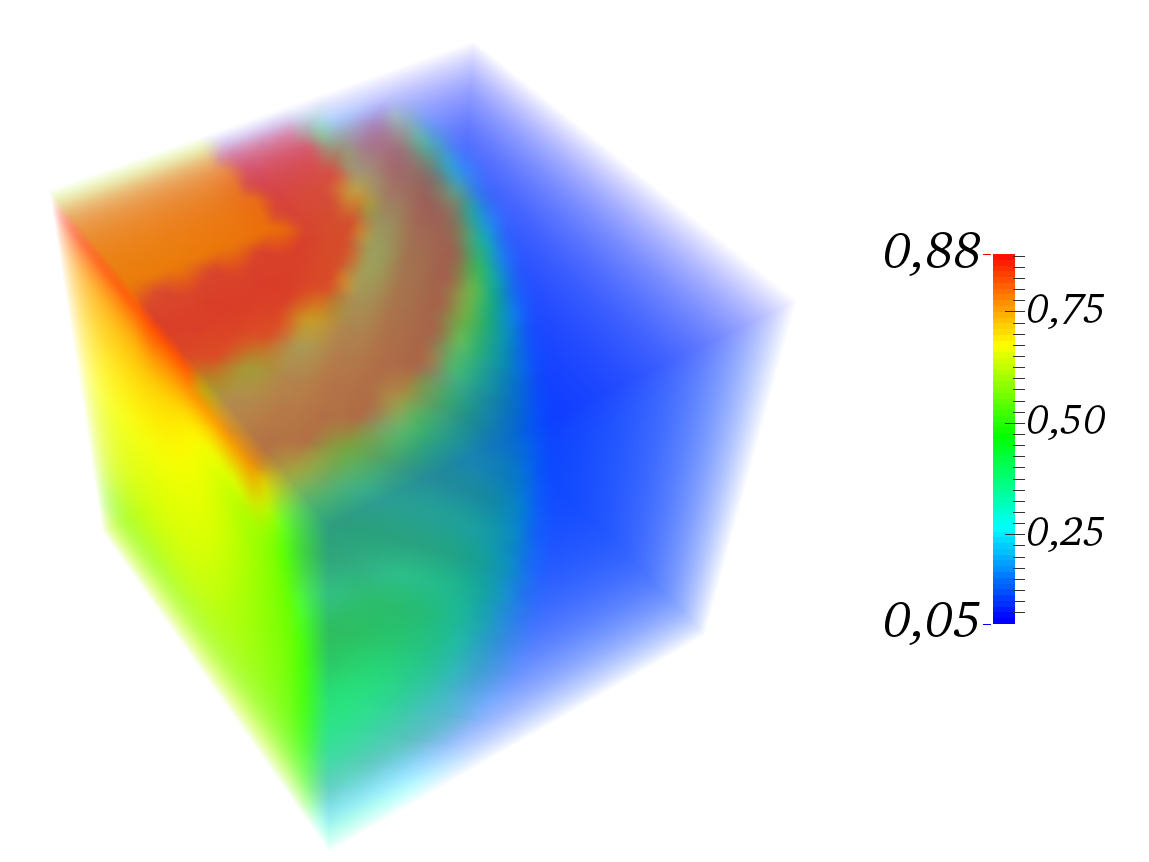
\includegraphics[width=1\textwidth]{test4/sw_1000.png}
       \vspace{1cm}
       \caption{Насыщенность $S_w$ в момент времени $t=1000$с}
    \end{minipage}
    \vspace{3cm}
    \vfill
    \begin{minipage}[h]{0.49\textwidth}
       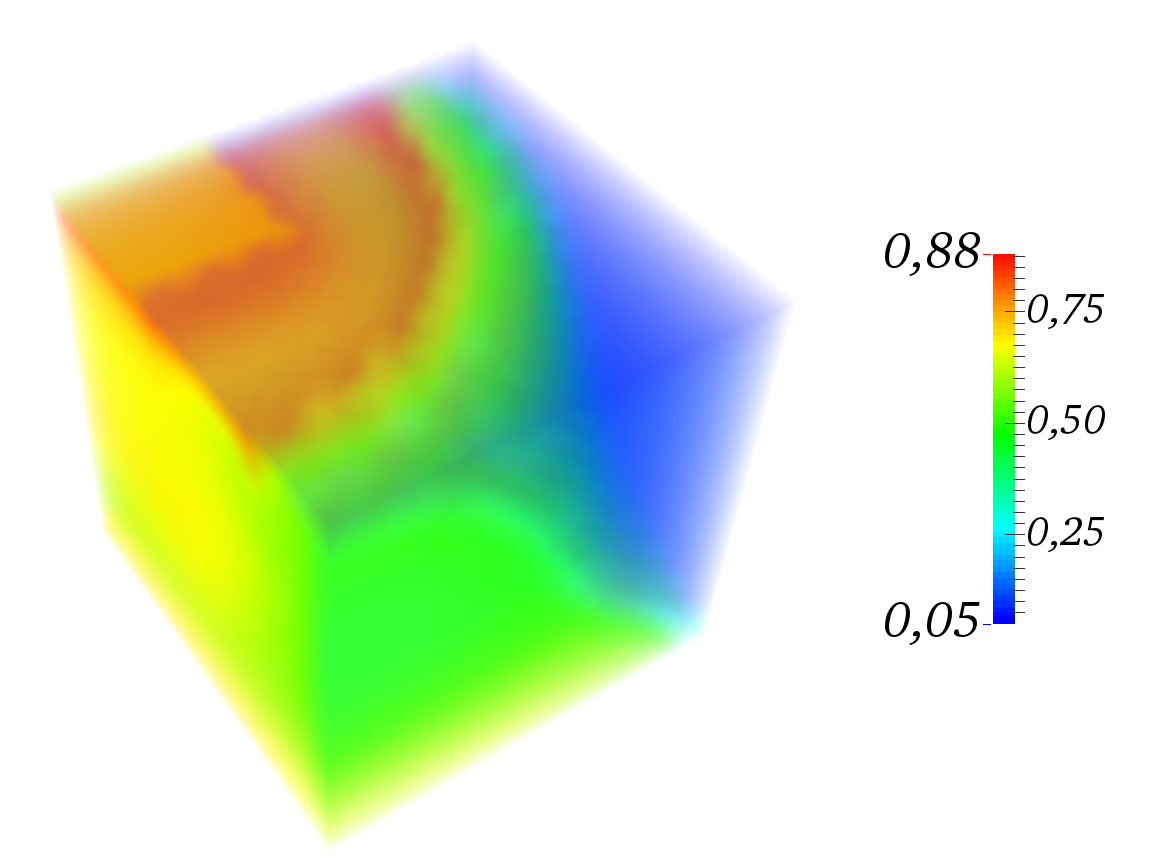
\includegraphics[width=1\textwidth]{test4/sw_2000.png}
       \vspace{1cm}
       \caption{Насыщенность $S_w$ в момент времени $t=2000$с}
    \end{minipage}
    \hfill
    \begin{minipage}[h]{0.49\textwidth}
       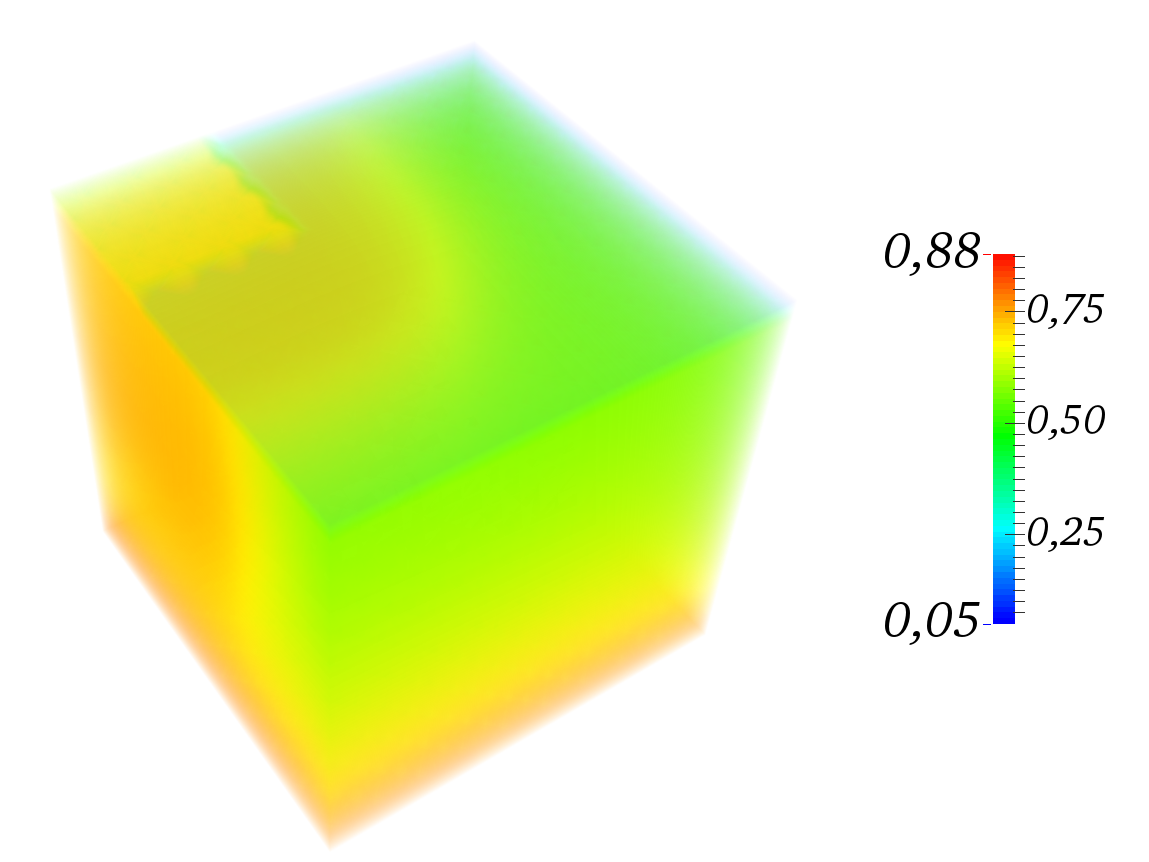
\includegraphics[width=1\textwidth]{test4/sw_6600.png}
       \vspace{1cm}
       \caption{Насыщенность $S_w$ в момент времени $t=6600$с}
    \end{minipage}
    \hfill  
  \end{center}
\end{figure}

\begin{figure}
  \begin{center}
    \begin{minipage}[h]{0.49\textwidth}
       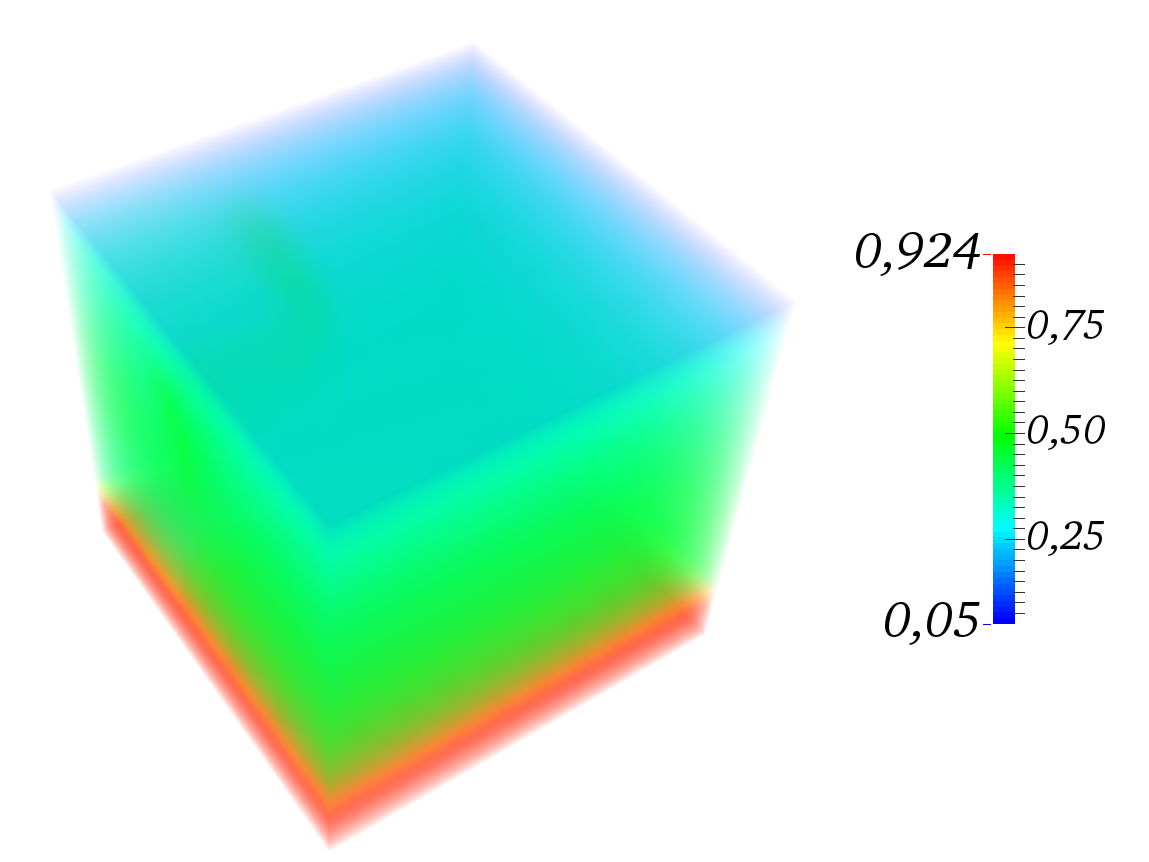
\includegraphics[width=1\textwidth]{test4/sn_200.png}
       \vspace{1cm}
       \caption{Насыщенность $S_n$ в момент времени $t=200$с}
    \end{minipage}
    \hfill
    \begin{minipage}[h]{0.49\textwidth}
       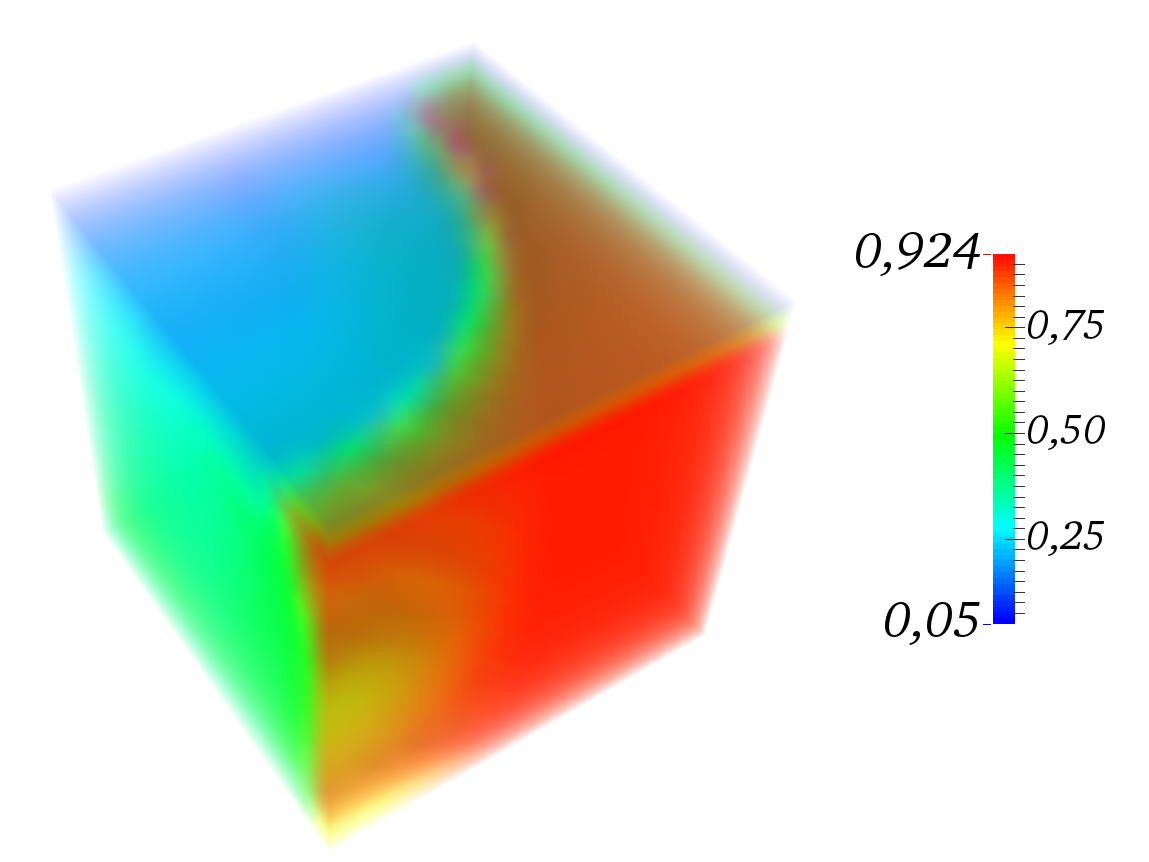
\includegraphics[width=1\textwidth]{test4/sn_1000.png}
       \vspace{1cm}
       \caption{Насыщенность $S_n$ в момент времени $t=1000$с}
    \end{minipage}
    \vspace{3cm}
    \vfill
    \begin{minipage}[h]{0.49\textwidth}
       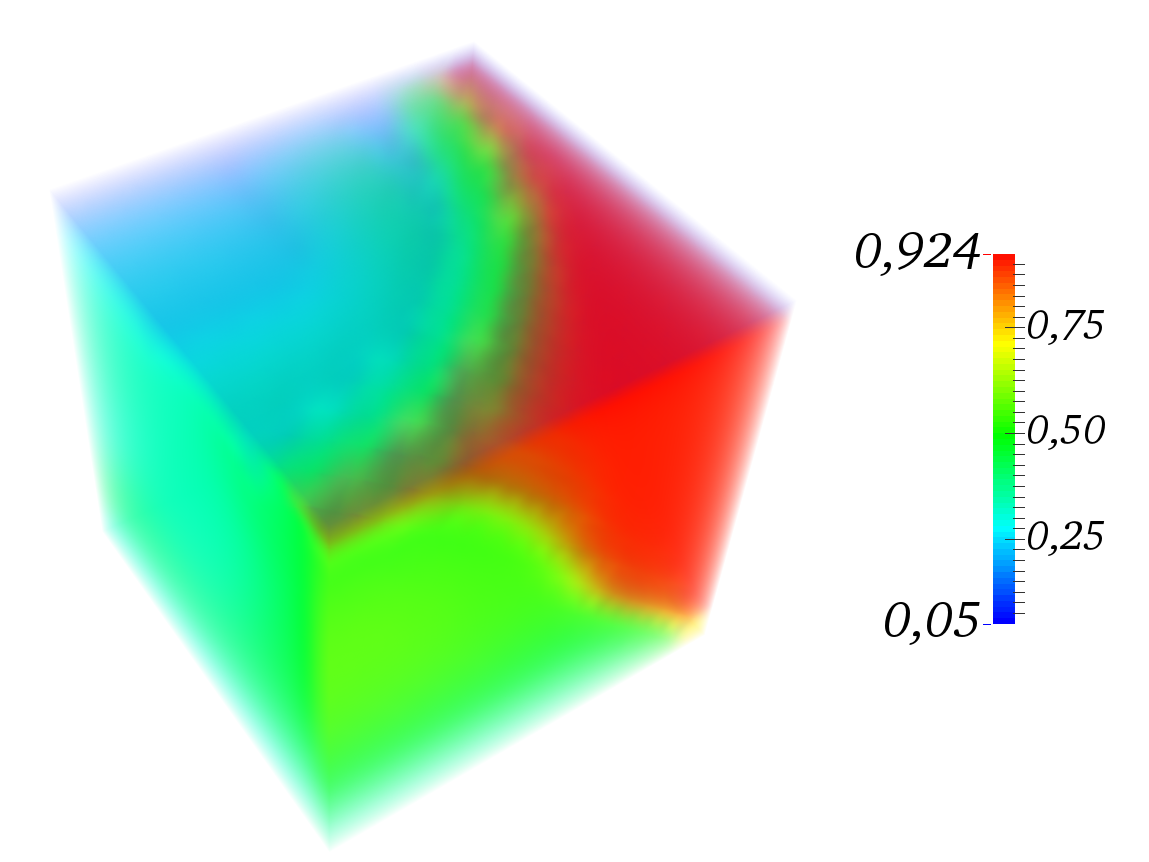
\includegraphics[width=1\textwidth]{test4/sn_2000.png}
       \vspace{1cm}
       \caption{Насыщенность $S_n$ в момент времени $t=2000$с}
    \end{minipage}
    \hfill
    \begin{minipage}[h]{0.49\textwidth}
       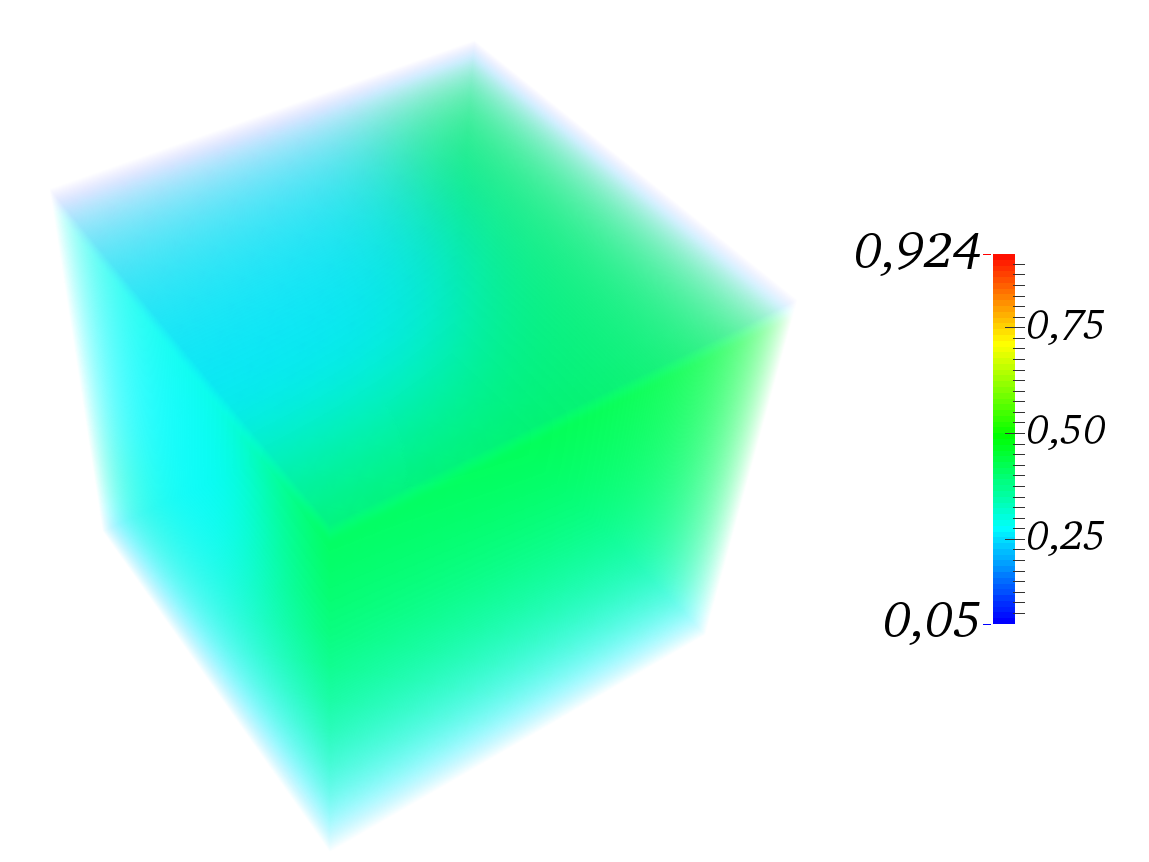
\includegraphics[width=1\textwidth]{test4/sn_6600.png}
       \vspace{1cm}
       \caption{Насыщенность $S_n$ в момент времени $t=6600$с}
    \end{minipage}
    \hfill  
  \end{center}
\end{figure}

\begin{figure}
  \begin{center}
    \begin{minipage}[h]{0.49\textwidth}
       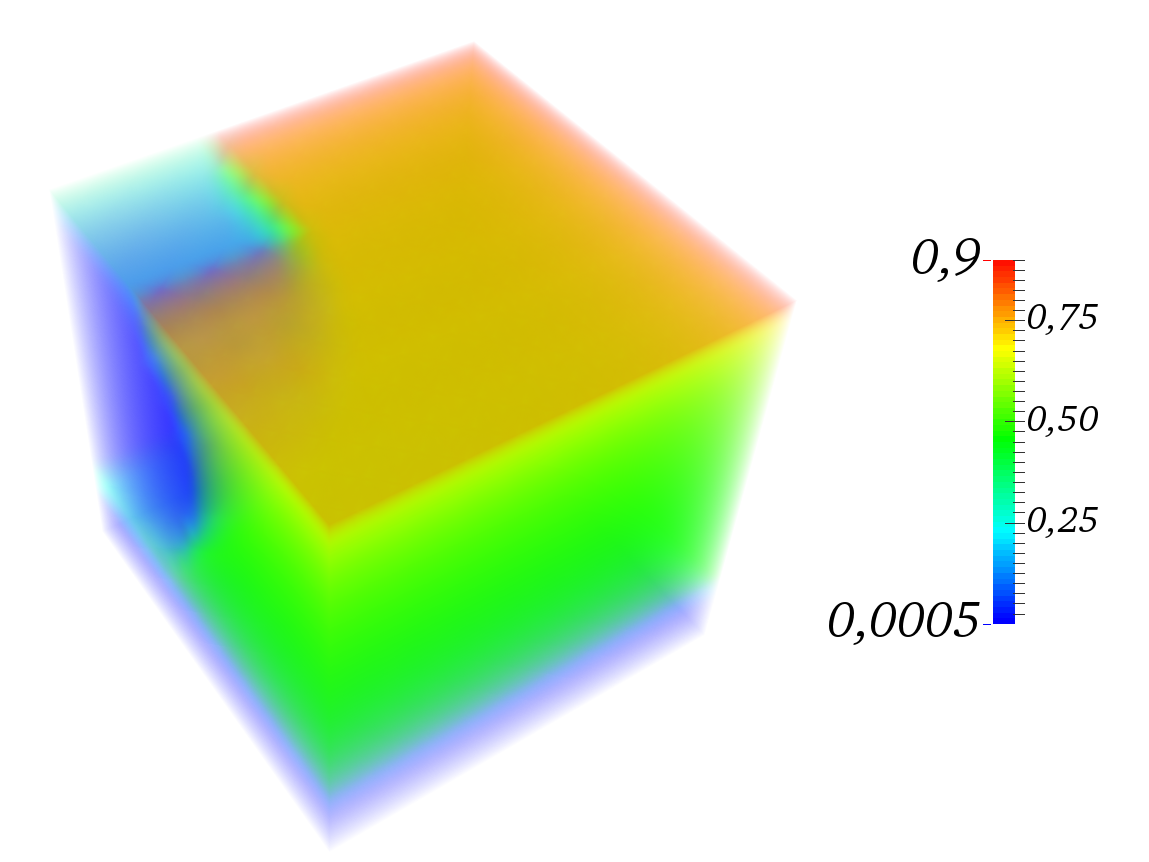
\includegraphics[width=1\textwidth]{test4/sg_200.png}
       \vspace{1cm}
       \caption{Насыщенность $S_g$ в момент времени $t=200$с}
    \end{minipage}
    \hfill
    \begin{minipage}[h]{0.49\textwidth}
       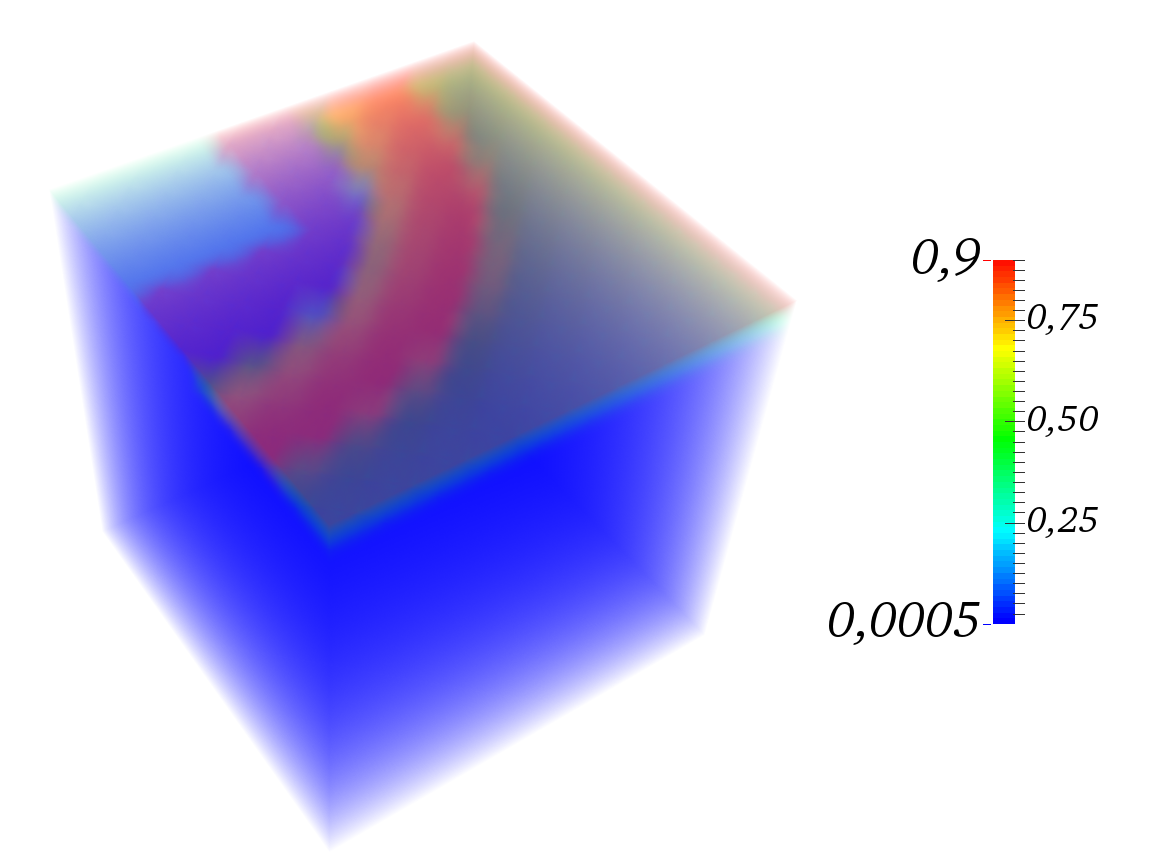
\includegraphics[width=1\textwidth]{test4/sg_1000.png}
       \vspace{1cm}
       \caption{Насыщенность $S_g$ в момент времени $t=1000$с}
    \end{minipage}
    \vspace{3cm}
    \vfill
    \begin{minipage}[h]{0.49\textwidth}
       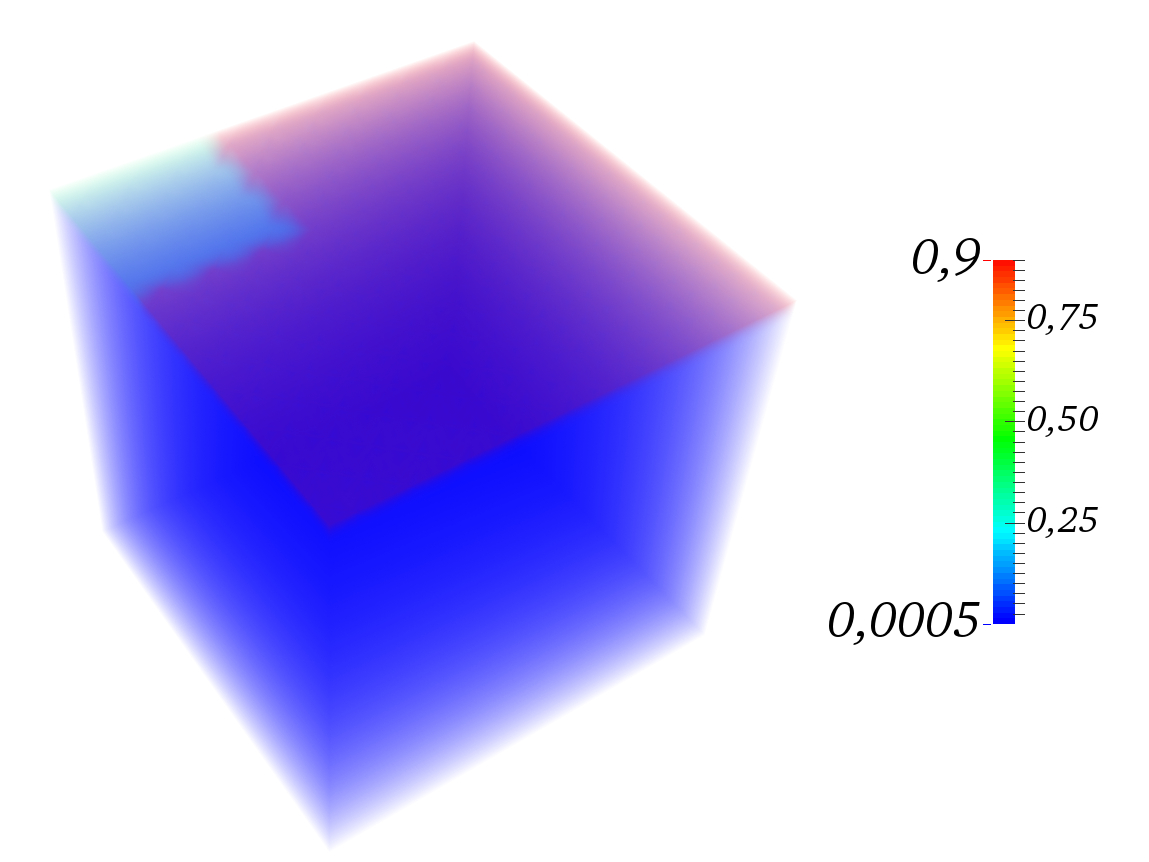
\includegraphics[width=1\textwidth]{test4/sg_2000.png}
       \vspace{1cm}
       \caption{Насыщенность $S_g$ в момент времени $t=2000$с}
    \end{minipage}
    \hfill
    \begin{minipage}[h]{0.49\textwidth}
       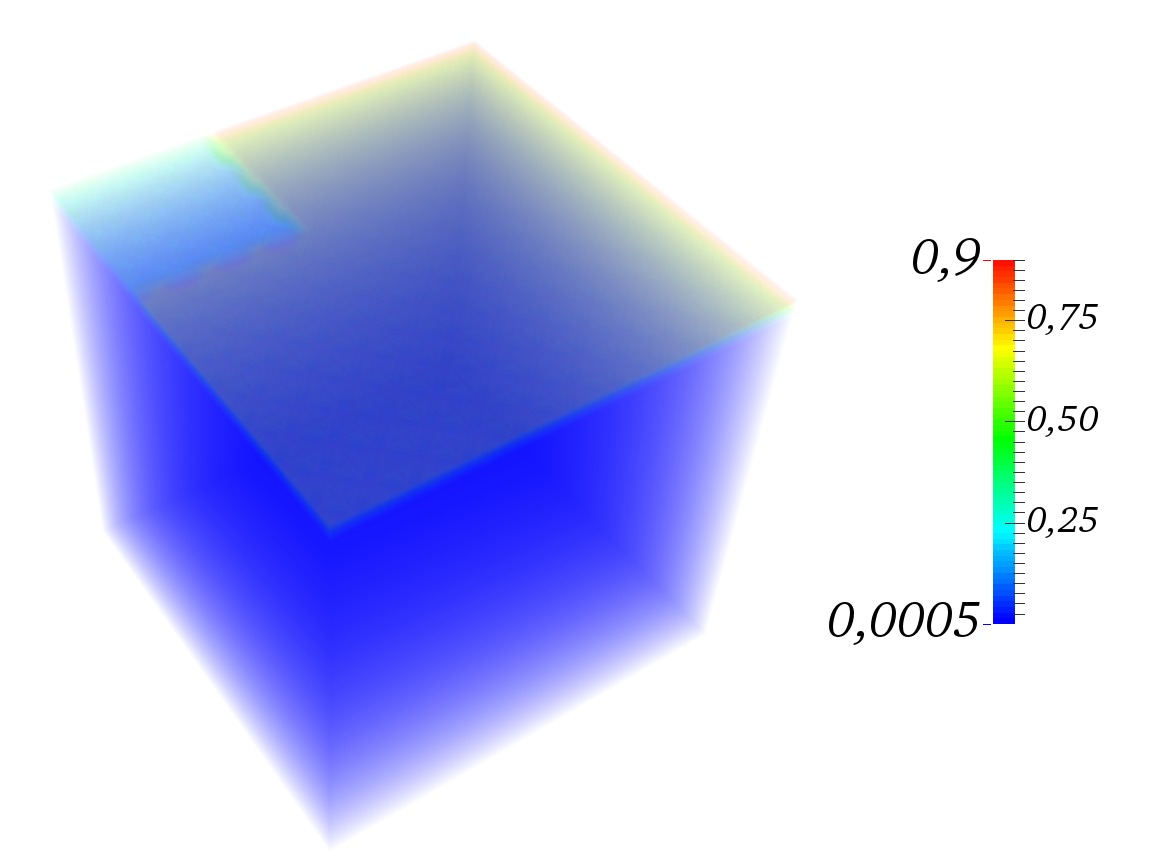
\includegraphics[width=1\textwidth]{test4/sg_6600.png}
       \vspace{1cm}
       \caption{Насыщенность $S_g$ в момент времени $t=6600$с}
    \end{minipage}
    \hfill  
  \end{center}
\end{figure}







